%*******10********20********30********40********50********60********70********80
\section{Constitutive Model}

A constitutive model for the concrete part at the mesoscale is used in this research since constitutive model in the macro scale cannot be applied to the mesoscale analysis.

In the analysis, the values of the material properties at the meso level given to the elements are actually different from the material properties where the object is analyzed at the macroscopic scale.

The material properties for the elements were determined to give the correct macroscopic properties.  In the discrete analysis done by Nagai et al. in 2005\cite{Nagai}, the shape and fineness of elements do affect the analysis results.

As we concern that the crack direction may affect the crack pattern, size of each concrete elements should be under consideration. Here for small example using 10x10x10mm model, the average diameter of elements is selected to be 0.05mm, while for larger size model in the dimension of 100x100x100mm, the size of each element is approximately 2x2x2mm to 3x3x3mm, almost the size of smallest coarse aggregate introduced. This assumption was made to represent the fracture behavior in concrete in a relatively high fineness and the behavior of both mortar and aggregate can be well presented.

In the elastic analysis, the relationship between macroscopic and mesoscopic Poisson's ratio, the effect of the mesoscopic Poisson's ratio on the macroscopic elastic modulus, are all confirmed by Nagai et al. in 2005\cite{Nagai}, using the same concepts.

\begin{equation}
  \begin{aligned}
  &\theta_{elem} = -24.8\theta^4+31.9\theta^3-16.4\theta^2 +4.28\theta\\
  &E_{elem} = (-33.7\theta_{elem}^4 + 17.0\theta_{elem}^3 - 4.13\theta_{elem}^2 + 0.327\theta_{elem} + 1)E
  \end{aligned}
\end{equation}

where E and $\theta$ are the macroscopic elastic modulus and Poisson's ratio of the analysis object, respectively.

The material characteristics of each component are presented by means of modeling springs. In normal spring, compressive and tensile stress ($\sigma$) are developed. Shear stress($\tau$) are developed by shear springs.

The elastic modulus of normal sprint($k_{nsp}$ and $k_{ssp}$) was presented in the previous chapter. For calculation of shear stress on 3D analysis, a resultant value of strains generated in two shear springs is adopted as shear strain in the constitutive model presented in this chapter. The strains and stress are calculated as follows:

\begin{equation}
  \begin{aligned}
  &\varepsilon = \frac{\delta_n}{h_1 + h_2}\\
  &\gamma = \frac{\delta_s}{h_1 + h_2}\\
  &\sigma = k_{nsp}\varepsilon\\
  &\tau = k_{ssp}\gamma
  \end{aligned}
\end{equation}

where $\varepsilon$ and $\gamma$ are the strain of normal and shear springs, respectively. $\delta_n$ and $\delta_s$ are the normal and shear relative displacement of elements of those springs, respectively.

In this study, the constitutive model of the concrete element has been developed based on simulations in material scale level. The constitutive models for the normal and shear springs of the concrete elements are shown in Figure \ref{fig:constitutive_model}.

\begin{figure}[ht!]
\centering
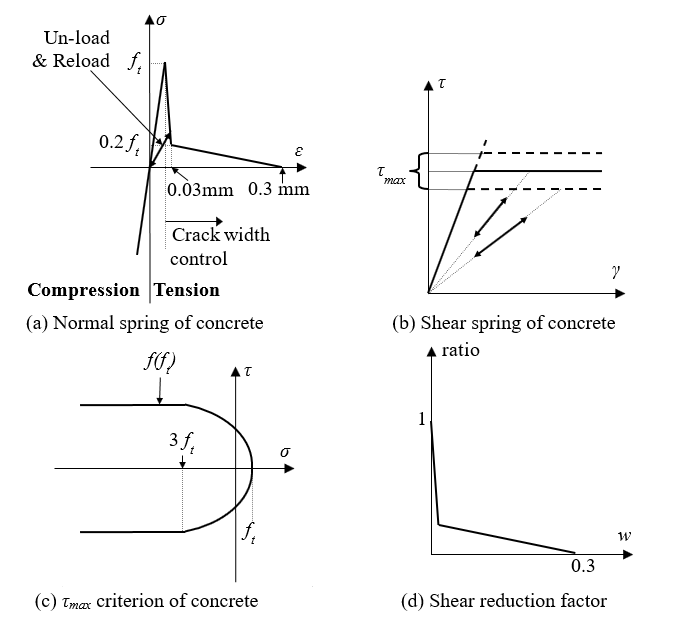
\includegraphics[width=.9\linewidth]{Files/Background/graph.png}
  \caption{Constitutive models of concrete}
  \label{fig:constitutive_model}
\end{figure}

The constitutive models of normal spring and a shear spring of concrete element using in this research are shown in Figure \ref{fig:constitutive_model}.

Basically, the concept of the concrete model is the same as the original simulation development by Nagai et al., 2005, where the compressive failure is not allowed at the mesoscale. In the tension zone, crack between two rigid bodies occurs only when the tensile stress of the normal spring exceeds the tensile strength of the concrete($f_t$). After exceeding the tensile strength($f_t$), the tensile stress of a normal spring is assumed to decrease bi-linearly, depending on the crack width, to zero at the maximum crack width($w_{max}$), which here is assumed as 0.3mm. An elasto-plastic behavior is also assumed when coming to the shear spring of concrete element with the$\tau_{max}$ is calculated based on the following equations:

\begin{equation}
  \begin{aligned}
  &\tau_{max} = \pm (1.6f_{telem}^2 (-\sigma + f_{telem})^0.4 + 0.15f_{telem}) if (\sigma \geq 3f_{telem})\\
  &\tau_{max} = \pm (1.6f_{telem}^2 (-3f_{telem} + f_{telem})^0.4 + 0.15f_{telem}) if (\sigma < 3f_{telem})
  \end{aligned}
\end{equation}

Besides, if fracture occurs in the normal spring, the calculated shear stress will be reduced according to the reduction of the normal stress. As a result, shear spring will now abole to carry the stress any longer when the crack width of the normal spring reaches $w_{max}$.
